% !TEX root = ../../main.tex

\section{Méthodes de résolution numérique en temps}
%%%%%%%%%%%%%%%%%%%%%%%%%%%%%%%%%%%%%%%%%%%%%%%%%%%%%%%%%%%%%%%%%%%%%%

Dans cette section nous allons présenter les principales méthodes utilisées pour résoudre numériquement des équations dites cinétiques en temps, et plus spécifiquement le système~\eqref{eq:0:vmhl:1}-\eqref{eq:0:vmhl:4}. Une fois discrétisé en $(\vb{x},\vb{v})$, les différents systèmes que nous regardons peuvent se réduire au modèle abstrait suivant :
\begin{equation}
  \dot{u}(t) = L(t,u) + N(t,u),\quad u(t=0)=u_0
  \label{eq:0:dtu}
\end{equation}
d'inconnue $u\in\mathbb{R}^n$ et où $L$ et $N$ sont des fonctions $(t,u)\in\mathbb{R}_+\times\mathbb{R}^n\mapsto\mathbb{R}^n$, $n\in\mathbb{N}$ est le nombre de dimensions, ou d'inconnues du problème. C'est sur cette équation~\eqref{eq:0:dtu} que nous allons présenter les différentes méthodes d'intégration en temps utilisées ici.

% --------------------------------------------------------------------
\subsection{Méthode de \emph{splitting} hamiltonien}
% --------------------------------------------------------------------

Les méthodes de \emph{splitting} sont classiquement utilisées dans la résolution d'équations cinétiques (\cite{Morrison:2017,Grandgirard:2006,Tronci:2010,Tronci:2014}), elles consistent à diviser l'équation à résoudre en plusieurs parties. La construction de ces méthodes en temps se fait par concaténation des différentes étapes en formant des palindromes.

Une méthode de \emph{splitting} consiste à résoudre les deux équations suivantes successivement :
\begin{eqnarray}
    \dot{u} = L(t,u) \label{eq:0:split:1}\\
    \dot{u} = N(t,u) \label{eq:0:split:2}
\end{eqnarray}
La solution de l'équation~\eqref{eq:0:dtu} au temps $t$ est $\varphi_t(u_0)$, et sera approchée par une composition de $\varphi_t^{[L]}(u_0)$ et $\varphi_t^{[N]}(u_0)$, respectivement solutions de~\eqref{eq:0:split:1} et~\eqref{eq:0:split:2}. Ainsi la méthode de Lie, \emph{splitting} d'ordre 1, consiste à approcher $\varphi_t(u_0)$ par $\varphi_t(u_0)\approx \varphi_t^{[L]} \circ \varphi_t^{[N]}(u_0)$. Si la résolution de chaque sous-système $\varphi_t^{[L]}$ et $\varphi_t^{[N]}$ est exacte, la seule erreur en temps provient du \emph{splitting}.

La résolution de chaque sous-système peut se faire sur des intervalles de temps différents (que nous noterons en indice), ainsi la méthode de Strang~\cite{Strang:1968}, \emph{splitting} d'ordre 2, s'écrit comme :
$$
  u(t) = S_{t}(u_0) = \varphi^{[L]}_{t/2}\circ\varphi^{[N]}_{t}\circ\varphi^{[L]}_{t/2}(u_0)
$$

Lorsque l'équation met en jeu plusieurs termes, comme c'est le cas pour le système~\eqref{eq:0:vmhl:1}-\eqref{eq:0:vmhl:4}, il est difficile de savoir comment choisir $L$ et $N$. L'hamiltonien du système permet de suggérer une décomposition intéressante, et de construire des méthodes appelées \emph{splitting} hamiltonien. \Josselin{voir dans \cite{Hairer:2006} s'il est nécessaire de résoudre exactement chaque sous-système pour avoir une splitting hamiltonien.}


\subsection{Méthode de type Runge-Kutta}
% --------------------------------------------------------------------

Les méthodes de type Runge-Kutta sont des méthodes d'approximation de solutions d'équations différentielles, développées dès 1901. Elles peuvent être vues comme une extension, à des ordres supérieurs, de la méthode d'Euler. Nous utiliserons ce type de méthodes pour résoudre la discrétisation en temps. Nous allons présenter ce type de méthode sur l'équation :
$$
  \dot{u} = N(t,u)
$$
où $u\in\mathbb{R}^n$, et $N:(t,u)\in\mathbb{R}_+\times\mathbb{R}^n\mapsto N(t,u)\in\mathbb{R}^n$ une fonction agissant sur $u$ et pouvant dépendre du temps $t$. Il s'agit d'un cas particulier de l'équation~\eqref{eq:0:dtu} où $L$ est la fonction nulle. Nous résumerons les méthodes par leur tableau de Butcher\cite{Butcher:2008}, qui se représentent sous la forme :
\begin{equation}  
  \begin{array}{c|c}
    \begin{matrix}
      c_1 \\
      \vdots \\
      c_s
    \end{matrix}
    &
    \begin{matrix}
      a_{11} & \cdots & a_{1s} \\
      \vdots & \ddots & \vdots \\
      a_{s1} & \cdots & a_{ss}
    \end{matrix} \\
    \hline
     & \begin{matrix} b_1 & \cdots & b_s \end{matrix} \\
  \end{array}
  \label{eq:0:butcher}
\end{equation}
et qui se lit :
$$
  \begin{aligned}
    u^{(i)} &= u^n + \Delta t \sum_{j=1}^s a_{ij} N(t^n+c_j\Delta t,u^{(j)}) \\
    u^{n+1} &= u^n + \Delta t \sum_{i=1}^s b_i N(t^n+c_i\Delta t, u^{(i)}),
  \end{aligned}
$$
où $u^n\approx u(t^n)$ avec $t^n=n\Delta t$, et où $\Delta t$ est le pas de temps.

Nous n’étudierons, pour des raisons de performances numériques, que des méthodes dites explicites, c'est-à-dire que chaque étage ne nécessite que les étages précédents pour être calculé. Dans ce cas, la matrice $(a_{ij})_{i,j}$ est triangulaire strictement inférieure. Dans le cadre de méthode explicite, il est possible de convertir la méthode, comme la méthode RK(3,3) de Shu-Osher, pour n'avoir qu'une seule évaluation de la fonction non linéaire $N$ par étage de la méthode.

Un intérêt des méthodes de type Runge-Kutta explicite est la montée en ordre. En effet celle-ci peut se faire de manière presque linéaire par rapport au nombre d'étages. À l'inverse, ces méthodes ne préservent pas l'énergie du système qu'elles résolvent, la montée en ordre est donc une nécessité pour réduire l'erreur et garantir la validité des résultats. Un autre inconvénient de ce type de résolution est l'introduction de condition de stabilité, que nous détaillerons un peu plus dans le cadre du chapitre~\ref{chap1}.

Nous bénéficions de la large littérature sur le sujet des méthodes de type Runge-Kutta, l'étude de stabilité ou de convergence (voir~\cite{Shu:2001,Butcher:2008,Gottlieb:2011,Baldauf:2008,Spiteri:2002}), ainsi que des améliorations dans des contextes spécifiques ; telles que les méthodes de Dormand-Prince permettant des stratégies de pas de temps adaptatifs (voir~\cite{Dormand:1978,Dormand:1980,,Gustafsson:1988,,Gustafsson:1994,Balac:2013,Balac:2014}), ou les méthodes de Lawson qui profitent de la structure linéaire de l'équation (voir~\cite{Lawson:1967,Isherwood:2018,Hochbruck:2020}).

\subsubsection{Méthode de Lawson}
% --------------------------------------------------------------------

Les méthodes de Lawson sont une optimisation des méthodes de type Runge-Kutta à des équations ayant une partie linéaire que l'on écrit comme suit :
$$
  \dot{u}(t) = Lu(t) + N(t,u)
$$
il s'agit du cas particulier de l'équation~\eqref{eq:0:dtu} où $L$ est une matrice ou un opérateur linéaire agissant sur $u$. Le principe de la méthode de Lawson est d'utiliser une formule de Duhamel sur $u$ pour résoudre exactement le terme linéaire. Ceci permet de se soustraire d'une condition de stabilité provenant du terme linéaire, et réduire l'erreur en résolvant exactement le plus de termes possibles.

Nous effectuons une formule de Duhamel en notant $v = e^{-tL}u$, ce qui nous permet de calculer :
$$
  \dot{v}(t) = -Le^{-tL}u(t) + e^{-tL}\dot{u}(t)
$$
d'où :
$$
  \dot{v}(t) = -Le^{-tL}u(t) + e^{-tL}Lu(t) + e^{-tL}N(t,u).
$$
On peut maintenant écrire l'équation sur $v$ que nous souhaitons résoudre avec une méthode de type Runge-Kutta :
$$
  \dot{v} = \tilde{N}(t,v)
$$
avec $\tilde{N}:(t,v)\in\mathbb{R}_+\times\mathbb{R}^n\mapsto e^{-tL}N(t,e^{tL}v)\in\mathbb{R}^n$. La méthode de Lawson consiste à réécrire la méthode Runge-Kutta sur $v$ en la variable $u$, où la partie linéaire est résolue exactement. La méthode de Lawson, induite par une méthode Runge-Kutta explicite décrite par le tableau de Butcher~\eqref{eq:0:butcher}, s'écrit alors :
$$
  \begin{aligned}
    u^{(i)} &= e^{c_i\Delta t L}u^n + \Delta t \sum_{j=1}^{i-1} a_{ij}e^{-(c_j-c_i)\Delta t L}N(t^n+c_j\Delta t,u^{(j)}) \\
    u^{n+1} &= e^{\Delta t L}u^n + \Delta t \sum_{i=1}^{s} b_i e^{(1-c_i)\Delta tL} N(t^n+c_i\Delta t,u^{(i)})
  \end{aligned}
$$

Comme pour une méthode Runge-Kutta classique, il est possible d'appliquer la même méthode d'optimisation de Shu-Osher pour n'avoir qu'une seule évaluation de la fonction non-linéaire $N$ par étage dans le cadre d'une méthode explicite.


\section{Méthodes de résolution numérique en espace}
%%%%%%%%%%%%%%%%%%%%%%%%%%%%%%%%%%%%%%%%%%%%%%%%%%%%%%%%%%%%%%%%%%%%%%

Nous présentons dans cette section les méthodes numériques permettant de discrétiser en espace ($\vb{x}$ ou $\vb{v}$) que nous allons utiliser pour résoudre numériquement le système~\eqref{eq:0:vmhl:1}-\eqref{eq:0:vmhl:4}.

% --------------------------------------------------------------------
\subsection{Méthode WENO}
% --------------------------------------------------------------------

La méthode WENO, pour \emph{Weighted Essentially Non-Oscillatory}, est une méthode volumes finis ou différences finies, dont l'écriture classique est d'ordre 5. Il s'agit d'une méthode \emph{upwind}, d'ordre élevé, combinée à des poids non-linéaires permettant de réduire les oscillations par de la baisse d'ordre et de la diffusion numérique. La méthode d'ordre 5 est présentée dans \cite{Liu:1994,Jiang:1996,Shu:1999,Shu:2003}. Nous la présentons ici pour une équation de transport de la forme :
$$
  \partial_t u + \partial_x f(u) = 0,\qquad u(t=0,x) = u_0(x)
$$
avec $u(t,x)$ la fonction inconnue dépendant du temps $t\geq 0$ et de l'espace $x\in\Omega$ (supposé ici périodique par commodité), et $f:u\mapsto f(u)$ une fonction agissant sur $u$. On définit une discrétisation de l'espace $x_i = i\Delta x + x_0$, $i=0,\dots,N_x$, avec $\Delta x>0$ le pas d'espace. La méthode WENO se présente comme suit :
$$
  \partial_t u_j(t) + \frac{1}{\Delta x}\left( \hat{f}_{j+\frac{1}{2}} - \hat{f}_{j-\frac{1}{2}} \right) = 0,
$$
où $u_j(t)\approx u(t,x_j)$, $j=0,\dots,N$, et où $\hat{f}_{j+\frac{1}{2}} = \hat{f}(u_{j-2},\dots,u_{j+2})$ est le flux numérique, ici présenté pour WENO5, avec $(u_{j-2},\dots,u_{j+2})$ le \emph{stencil} de la méthode, c'est-à-dire le voisinage de points nécessaire pour calculer une approximation de la dérivée en espace. Comme pour une méthode \emph{upwind}, il est nécessaire de distinguer le flux en deux parties, positive et négative :
$$
  f(u) = f^+(u) + f^-(u).
$$
Pour cela il est possible d'utiliser le flux de Lax-Friedrichs (voir~\cite{Shu:1997}). Dans les cas qui nous intéressent, $f:u\mapsto au$ est une fonction linéaire, il est donc simplement nécessaire de connaître le signe de la vitesse d'advection $a$, on note alors $a^+ = \max(a,0)$ et $a^-=\min(a,0)$ et on a $f^\pm_j=f^\pm(u_j)=a^\pm u_j$.

\begin{figure}[h]
  \centering
  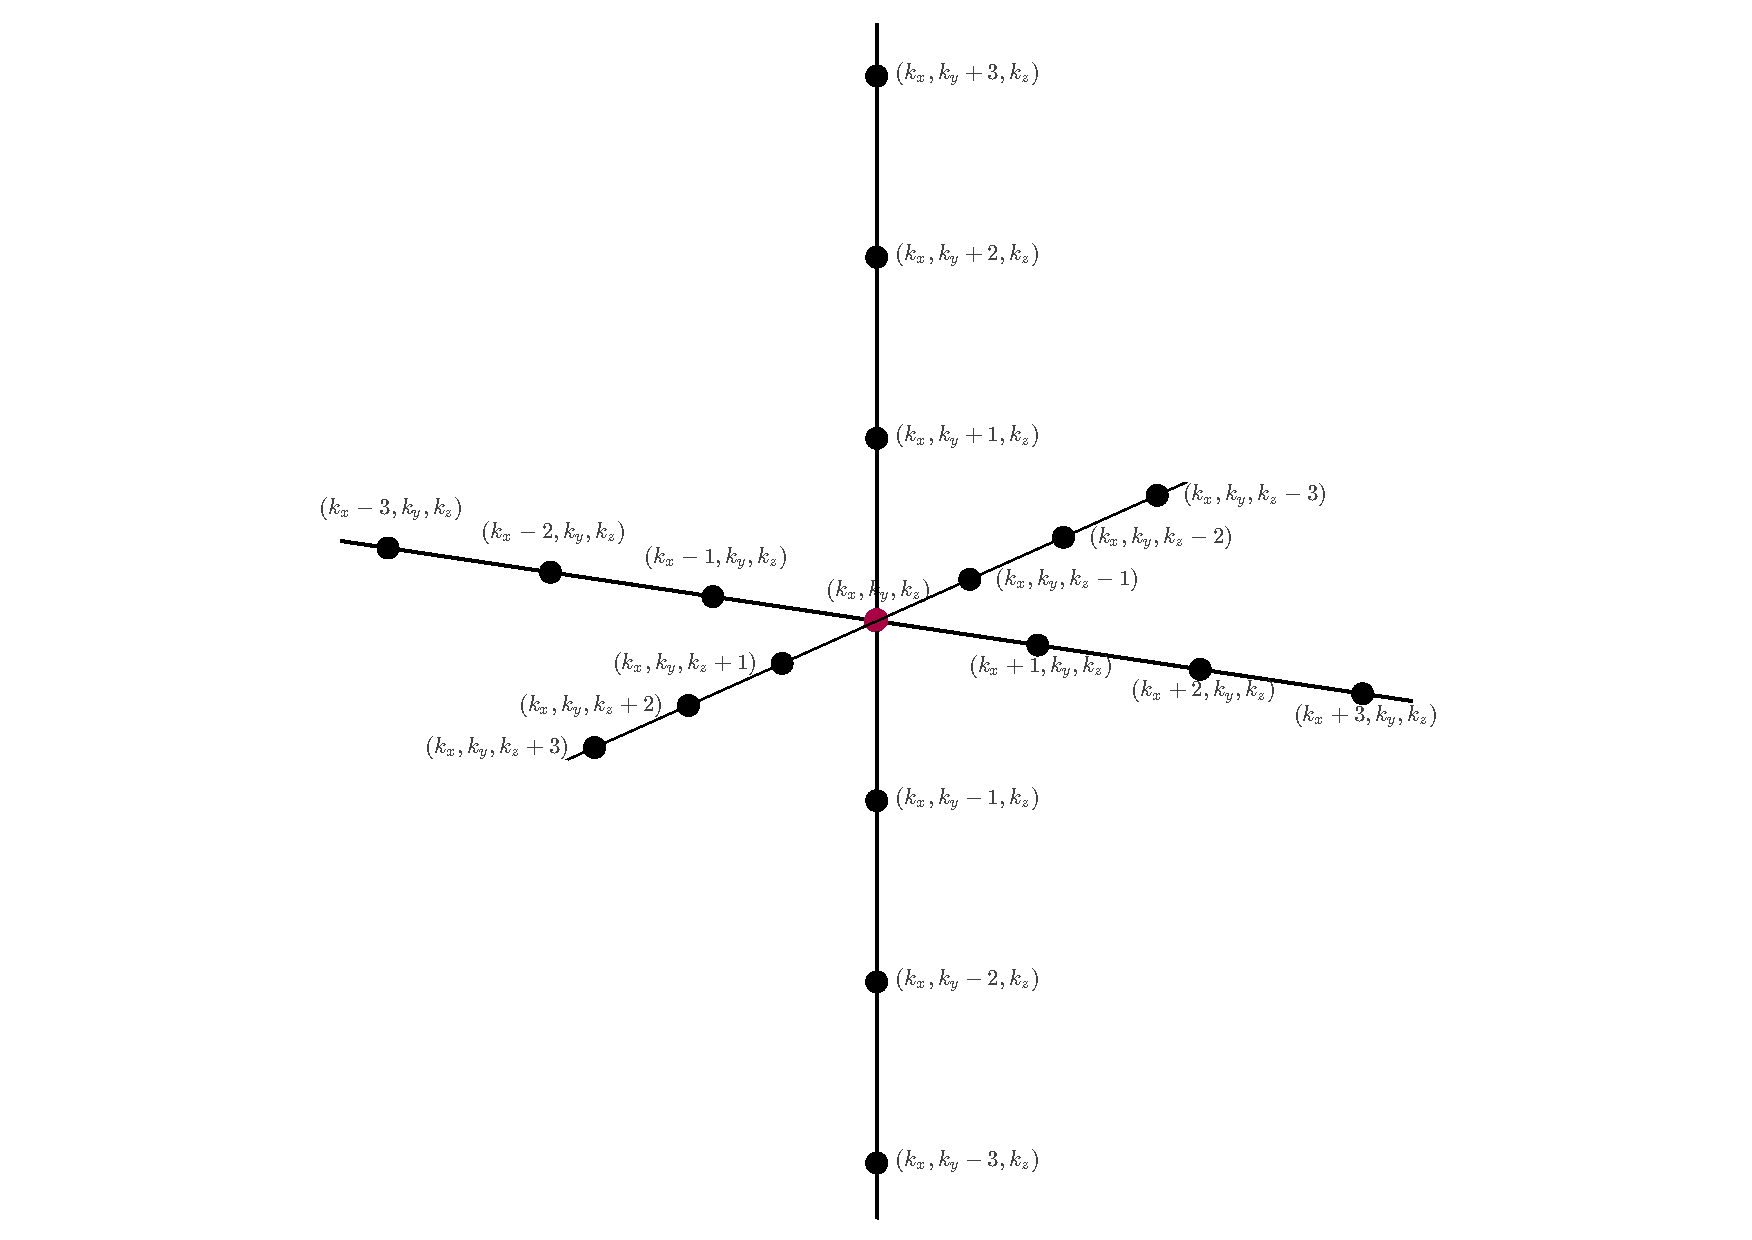
\includegraphics[width=0.9\textwidth]{\localPath/figures/stencil.pdf}
  \caption{Présentation des \emph{stencils} utilisés par la méthode WENO5 pour calculer le flux numérique.}
  \label{fig:intro:stencil}
\end{figure}

La méthode WENO5 consiste en 3 interpolations, sur 3 \emph{stencils} différents, comme l'illustre la figure~\ref{fig:intro:stencil}, pondérées par des poids non-linéaires issus des approximations des dérivées successives de $f$. L'écriture des poids s'effectue comme suit dans le cas $f^-=0$ :
$$
  \begin{aligned}
    \beta_0 &= \frac{13}{12}( \underbrace{f^+_{j-2} - 2f^+_{j-1} + f^+_{j}}_{\Delta x^2(f''_{j} + \mathcal{O}(\Delta x))})^2   + \frac{1}{4}( \underbrace{  f^+_{j-2} - 4f^+_{j-1} + 3f^+_{j}  }_{ 2\Delta x ( f'_{j} + \mathcal{O}(\Delta x^2))})^2 \\
    \beta_1 &= \frac{13}{12}( \underbrace{f^+_{j-1} - 2f^+_{j}   + f^+_{j+1}}_{\Delta x^2(f''_{j} + \mathcal{O}(\Delta x^2))} )^2 + \frac{1}{4}( \underbrace{  f^+_{j-1} -               f^+_{j+1}}_{ 2\Delta x   f'_{j} + \mathcal{O}(\Delta x^2))})^2 \\
    \beta_2 &= \frac{13}{12}( \underbrace{f^+_{j}   - 2f^+_{j+1} + f^+_{j+2}}_{\Delta x^2(f''_{j} + \mathcal{O}(\Delta x))} )^2   + \frac{1}{4}( \underbrace{ 3f^+_{j}   - 4f^+_{j+1} +  f^+_{j+2}}_{-2\Delta x ( f'_{j} + \mathcal{O}(\Delta x^2))})^2 \\
  \end{aligned}
$$
où les coefficients $\beta_0$ sont appelés indicateurs de continuité (\emph{indicators of smoothness}). Ce qui nous permet de calculer les poids définis par :
$$
  \alpha_i = \frac{\gamma_i}{(\varepsilon + \beta_i)^2},\quad i=0,1,2
$$
où $\varepsilon$ est un paramètre numérique pour assurer la non nullité du dénominateur, il sera pris à $10^{-6}$ ; et avec $\gamma_0=\frac{1}{10}$, $\gamma_1=\frac{6}{10}$ et $\gamma_2=\frac{3}{10}$. La normalisation des poids s'effectue comme suit :
$$
  w_i = \frac{\alpha_i}{\sum_m \alpha_m},\quad i=0,1,2
$$
Nous pouvons ensuite calculer les flux numériques pour WENO5 \cite{Shu:2003}, donnés par :
$$
  \begin{aligned}
    \hat{f}_{j+\frac{1}{2}}^+   =\ & w_0\left(  \frac{2}{6}f^+_{j-2} - \frac{7}{6}f^+_{j-1} + \frac{11}{6}f^+_{j}   \right)
                                +    w_1\left( -\frac{1}{6}f^+_{j-1} + \frac{5}{6}f^+_{j}   +  \frac{2}{6}f^+_{j+1} \right) \\
                                +  & w_2\left(  \frac{2}{6}f^+_{j}   + \frac{5}{6}f^+_{j+1} -  \frac{1}{6}f^+_{j+2} \right).
  \end{aligned}
$$
La méthode WENO5 prend la forme finale :
$$
  \partial_xf(x_j) \approx \frac{1}{\Delta x}\left[ \left(\hat{f}_{j+\frac{1}{2}}^+ - \hat{f}_{j-\frac{1}{2}}^+ \right) + \left(\hat{f}_{j+\frac{1}{2}}^- - \hat{f}_{j-\frac{1}{2}}^- \right) \right].
$$

Il existe des variantes de la méthode WENO5, permettant de réduire la perte d'ordre à l'approche d'un choc, à savoir WENO-M (\cite{Henrick:2005}) ou WENO-Z (\cite{Borges:2008}). Ces variations se font sur le calcul des poids non-linéaires. Ainsi la méthode WENO-M utilise une fonction de \emph{mappage} pour équilibrer les poids et est définie par :
$$
  \begin{aligned}
    \alpha_i    &= \frac{\gamma_i}{(\epsilon + \beta_i)^2} \\
    \tilde{w}_i &= \frac{\alpha_i}{\sum_k \alpha_k} \\
    g_i         &= w_i\left( \frac{\gamma_i + \gamma_i^2 - 3w_i\gamma_i + w_i^2}{\gamma_i^2 + w_i(1-2\gamma_i)} \right) \\
    w_i         &= \frac{g_i}{\sum_k g_k}
  \end{aligned}
$$
avec le paramètre $\epsilon = 10^{-4}$. La méthode WENO-Z est quant à elle définie par :
$$
  \begin{aligned}
    \alpha_i &= \gamma_i\left( 1+ \frac{\tau_5}{\epsilon + \beta_i} \right) \\
    w_i      &= \frac{\alpha_i}{\sum_k \alpha_k}
  \end{aligned}
$$
avec les paramètres $\epsilon = 10^{-40}$ et $\tau_5 = \beta_0 - \beta_2$. Cette dernière méthode est celle qui réduit le plus la perte d'ordre à l'approche d'une discontinuité. L'étude approfondie de ces méthodes n'est pas envisagée dans ce travail car les solutions de la physique des plasmas ne présentent pas de discontinuités. Il est à noter que ces méthodes conservent la même linéarisation que le schéma WENO5 classique de Jiang et Shu~\cite{Jiang:1996}, ce qui permet d'y appliquer les résultats de stabilités obtenus dans le chapitre~\ref{chap1}.

Il est possible de monter en ordre en suivant les résultats dans~\cite{Wu:2021}, l'ordre 5 sera considéré comme suffisant dans la suite de ce travail.

L'étude de la stabilité de la méthode WENO5 couplée avec différentes méthodes de type Runge-Kutta pour la résolution en temps a été initiée dans~\cite{Wang:2007} où il a été démontré l'instabilité de la méthode couplée avec la méthode d'Euler explicite, il est nécessaire d'avoir au moins un étage supplémentaire permettant d'assurer la stabilité, ou d'utiliser une méthode d'ordre 3. Des estimations de stabilité et de conditions de stabilité ont par la suite été proposées dans \cite{Motamed:2010,Lunet:2017}. Une étude automatique de la stabilité est présentée dans~\cite{Crouseilles:2019b} qui constitue le chapitre~\ref{chap1} de ce document.

% --------------------------------------------------------------------
\subsection{Méthode semi-lagrangienne}
% --------------------------------------------------------------------

Une méthode très populaire pour la résolution numérique de l'équation de Vlasov, car les termes de transports sont linéaires, et que cette méthode n'introduit pas de contrainte de stabilité est la méthode semi-lagrangienne.

$$
  \partial_t u + a\partial_xu = 0
$$

\begin{figure}[h]
  \centering
  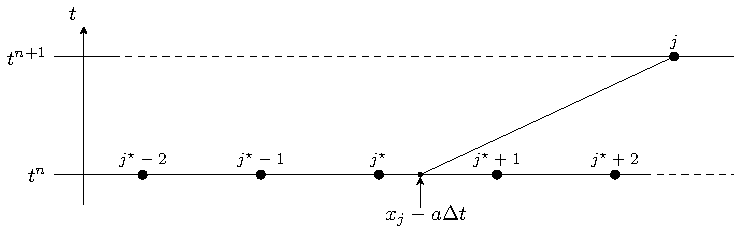
\includegraphics[width=0.9\textwidth]{\localPath/figures/semilag.pdf}
  \caption{Méthode des caractéristiques pour une méthode semi-lagrangienne avec une vitesse de transport $a>0$. \Josselin{En soit, la figure est de moi, je l'ai faite avec Tikz, je peux donc facilement la modifier au besoin.}}
  \label{fig:intro:semilag}
\end{figure}


% --------------------------------------------------------------------
\subsection{Méthode pseudo-spectrale}
% --------------------------------------------------------------------

Une autre méthode souvent utilisée pour la résolution d'équations aux dérivées partielles linéaires est la méthode pseudo-spectrale qui consiste dans notre cas à effectuer une transformée de Fourier discrète et ainsi transformer une dérivée dans l'espace réel en un produit dans l'espace de Fourier.

$$
  \hat{f} = \frac{1}{L}\int_0^L f(x)e^{-i\kappa x}\dd{x},\quad\kappa=\frac{2\pi}{L}n,\ n\in\mathbb{Z}
$$

